\clearpage
\section{Copper extension: operating perimeter and temporal validation}
\label{sec:copper-extension}

The original gold-only module omits copper. The separate extension adds the
three producing copper mines in Table~\ref{tab:copper-operating-perimeter};
the frozen gold operating vector and price/WACC draws remain identical in
the paired comparison. Copper mine statistics are already attributable:
ownership is recorded for interpretation and never multiplied again
\cite{barrick-mine-stats-2026}.

\begin{table}[H]
\centering\small
\caption{Copper scenario inputs from the three-month Q2 2026 mine tables;
volumes are already attributable \cite{barrick-mine-stats-2026}.}
\label{tab:copper-operating-perimeter}
\begin{tabularx}{\textwidth}{@{}Xrrrr@{}}
\toprule
Mine & Interest & Production (kt) & Sales (kt) & CoS (USD/lb) \\
\midrule
Lumwana & 100\% & 41 & 40 & 3.14 \\
Zald\'ivar & 50\% & 9 & 9 & 4.89 \\
Jabal Sayid & 50\% & 6 & 5 & 2.63 \\
\midrule
Total & & 56 & 54 & 3.39 reported \\
\bottomrule
\end{tabularx}
\end{table}

Lumwana is consolidated; Zald\'ivar and Jabal Sayid are equity-accounted
50\% interests. Their attributable operating contribution is included here,
although their revenue and CoS are outside consolidated copper totals
\cite{barrick-ar-2025}. The reported corporate CoS/lb is an attributable
metric and can differ from the mine-weighted value reconstructed from rounded
inputs. A consolidated-to-attributable cash/debt bridge therefore also applies
to the copper extension.

Sales and unit CoS are held at these Q2 levels for 20 quarters as a declared
scenario, not as fitted mine forecasts or guidance. The quarter's reported
capex and depreciation are retained as source facts; they are not separately
deducted or added in the CoS-margin experiment. Expansion schedules, Reko Diq,
reserves and closure liabilities require another operating/cash-flow model.
For price $C_t$ in USD/lb, sales $S_{i,t}$ in attributable kt and unit CoS
$c_{i,t}$ in USD/lb, the addition in USD millions is
\begin{equation}
\mathrm{CM}^{Cu}_t=\sum_i(C_t-c_{i,t})S_{i,t}
\frac{2204.6226218488}{1000}.
\label{eq:copper-margin}
\end{equation}
One kt is 1,000 tonnes; the factor converts kt to pounds then divides USD by
one million. The total gold-plus-copper margin is formed \emph{per path}
before the inherited tax/growth/ROIC transformation and quantiles. This is
after-CoS operating margin, not separately reconciled EBITDA or FCFF.

\paragraph{Copper price models and source dates.}
Standard COMEX HG futures and HXE American options are quoted in USD/lb;
every option's matching future is verified from its actual underlying
contract identifier. A 600-step constant-volatility futures tree estimates
American IV, then constructs equivalent European Black--76 quotes for the
European Heston, Bates and affine Hawkes engines. The 300/600-step difference
measures numerical discretisation sensitivity, not the error of stochastic
de-Americanisation. The four models have their own copper calibrations.

The initial 2 September static surface contains 88 real quotes, 76 eligible,
with 62 fitted and 14 reserved strikes. Those held-out strikes test
interpolation, not temporal OOS. The subsequent historical pilot samples ten
dates spanning July--September, using up to 112 spaced locations over expiries
75--250 days away. Quality filters require bid/ask validity, quote and future
age at most 120 seconds and relative spread at most 20\%. Only dates with
64 actual eligible quotes on at least three expiries enter temporal fitting.
No quotes are generated to meet the threshold. This fit uses all eligible
sampled quotes, rather than gold's fixed CC64 sample.

Each origin uses only its own options and an as-of Treasury curve; its
structural parameters are frozen while variance/intensity is projected to
the next admitted date. Target matching futures and dated rates condition
scoring. Common target support, origin-mean IV and persistence inside the
origin surface's convex hull are reported explicitly. This is conditional
IV-surface validation, not a physical price forecast. The current catalogue
has survivorship limits and IB does not return expired-option history
\cite{ib-historical-limitations}. Missing quotes and request timeouts are
separate findings; timeouts do not prove historical data absence.

\paragraph{Valuation boundary.}
Copper paths follow log-linear observed forward anchors at \emph{future
delivery dates}, holding the final level flat beyond support. Independence
is the base gold/copper scenario; terminal Gaussian-score dependence
$\pm0.5$ uses whole-path permutations preserving marginal distributions and
is not an estimated Brownian correlation. The primary comparison is five
years without terminal value; signed perpetuity is a separate sensitivity.
The comparison retains the inherited 20-quarter simulation grid, whose gold
vector starts with Q1--Q2 actuals although the option snapshot is 2 September.
It does not roll the operating calendar forward to exclude elapsed quarters.
That calendar reconciliation is required for a dated prospective DCF.
Neither conditional forwards nor IV tests validate physical five-year copper
prices, future mine sales, costs or corporate equity value.

\IfFileExists{chapters/generated/copper-results.tex}{%
\subsection{Completed historical pilot and paired operating-value results}
\label{sec:copper-completed-results}
The ten-date pilot admits 7 dates and 6 chronological pairs, with 480 common model forecasts and 375 observations on persistence support. Its gaps are the actual gaps between admitted dates, not assumed daily steps. The remaining 21 gold reference dates were not acquired in this pilot; their absence from this experiment does not establish unavailable history. The table records the quality exclusions rather than manufacturing a balanced panel.

\begin{table}[H]
\centering
\small
\caption{Actual copper pilot coverage; dates below 64 eligible quotes or three expiries are excluded.}
\label{tab:copper-temporal-coverage}
\begin{tabularx}{\textwidth}{@{}Xrrrr@{}}
\toprule
Date & Retrieved & Eligible & Expiries & Admitted \\
\midrule
2026-07-09 & 100 & 75 & 5 & Yes \\
2026-07-10 & 104 & 53 & 5 & No \\
2026-07-20 & 79 & 74 & 5 & Yes \\
2026-07-31 & 75 & 18 & 2 & No \\
2026-08-03 & 73 & 41 & 5 & No \\
2026-08-12 & 88 & 82 & 6 & Yes \\
2026-08-21 & 100 & 86 & 6 & Yes \\
2026-08-31 & 97 & 87 & 6 & Yes \\
2026-09-01 & 97 & 65 & 6 & Yes \\
2026-09-02 & 99 & 86 & 6 & Yes \\
\bottomrule
\end{tabularx}
\end{table}

Admitted origin--target pairs (calendar-day gaps): 2026-07-09 to 2026-07-20 (11); 2026-07-20 to 2026-08-12 (23); 2026-08-12 to 2026-08-21 (9); 2026-08-21 to 2026-08-31 (10); 2026-08-31 to 2026-09-01 (1); 2026-09-01 to 2026-09-02 (1).
The reported RMSE is the equal-weight mean of target-date RMSEs. The $R^2$ instead compares sums of target-date MSEs on each declared support. Root-mean MSE and observation-weighted pooled scores are retained separately in the reproducibility outputs.
\begin{table}[H]
\centering
\small
\caption{Copper conditional temporal IV tests: date-equal aggregation. The persistence comparison uses its inside-hull support; fixed-origin robustness freezes the first admitted fit.}
\label{tab:copper-temporal-models}
\begin{tabularx}{\textwidth}{@{}Xrrr@{}}
\toprule
Model & Rolling RMSE (bp) & $R^2_{mean}$ & $R^2_{persist}$ \\
\midrule
Black--76 & 106.48 & 0.002 & -1.294 \\
Heston & 71.46 & 0.458 & -0.422 \\
Bates--Poisson & 70.49 & 0.465 & -0.389 \\
Bates--Hawkes & 67.65 & 0.518 & -0.208 \\
\bottomrule
\end{tabularx}
\end{table}

\begin{table}[H]
\centering
\small
\caption{Fixed-first-origin robustness on the same 480 model forecasts; persistence support contains 333 observations. Structural parameters remain frozen at 2026-07-09.}
\label{tab:copper-fixed-origin}
\begin{tabularx}{\textwidth}{@{}Xrrr@{}}
\toprule
Model & Fixed RMSE (bp) & $R^2_{mean}$ & $R^2_{persist}$ \\
\midrule
Black--76 & 115.38 & 0.001 & -0.345 \\
Heston & 111.94 & -0.050 & -0.282 \\
Bates--Poisson & 90.94 & 0.337 & 0.193 \\
Bates--Hawkes & 92.56 & 0.334 & 0.182 \\
\bottomrule
\end{tabularx}
\end{table}

In the rolling test, no model improves on observed-surface persistence on its common support. The fixed-origin check gives positive persistence-relative point estimates for Bates--Poisson (0.193), Bates--Hawkes (0.182); its different origin gaps and support do not establish stable superiority. Reserved-strike interpolation results remain a separate experiment. Fixed-origin targets overlap the rolling sample and do not constitute independent replication. With only 6 forecast pairs, these estimates support a preliminary diagnostic, not a stable economic model ranking or a claim of statistical superiority.

\begin{table}[H]
\centering
\small
\caption{Paired five-year operating-value proxies, USD billion, no terminal value, independent gold/copper scenarios and 8,192 common paths. Monte Carlo SE concerns only the mean increment.}
\label{tab:copper-paired-value}
\begin{tabularx}{\textwidth}{@{}Xrrrr@{}}
\toprule
Model & Gold only & Gold + copper & Increment & MC SE \\
\midrule
Black--76 & 14.857 & 17.484 & 2.627 & 0.023 \\
Heston & 14.847 & 17.465 & 2.618 & 0.039 \\
Bates--Poisson & 14.746 & 17.409 & 2.663 & 0.040 \\
Bates--Hawkes & 14.776 & 17.417 & 2.641 & 0.037 \\
\bottomrule
\end{tabularx}
\end{table}

The valuation uses a full eligible 2 September copper fit with that date's Treasury curve. Its parameters are used only in the final scenario, not retroactively in historical origins. The gold baseline remains frozen, including its company-actual/eight-mine-forecast scope break. Parameter uncertainty, operating-plan uncertainty and the unreconciled corporate cash-flow bridge are outside the Monte Carlo SE. A temporal IV test does not validate those missing economic quantities.

\begin{figure}[H]
\centering
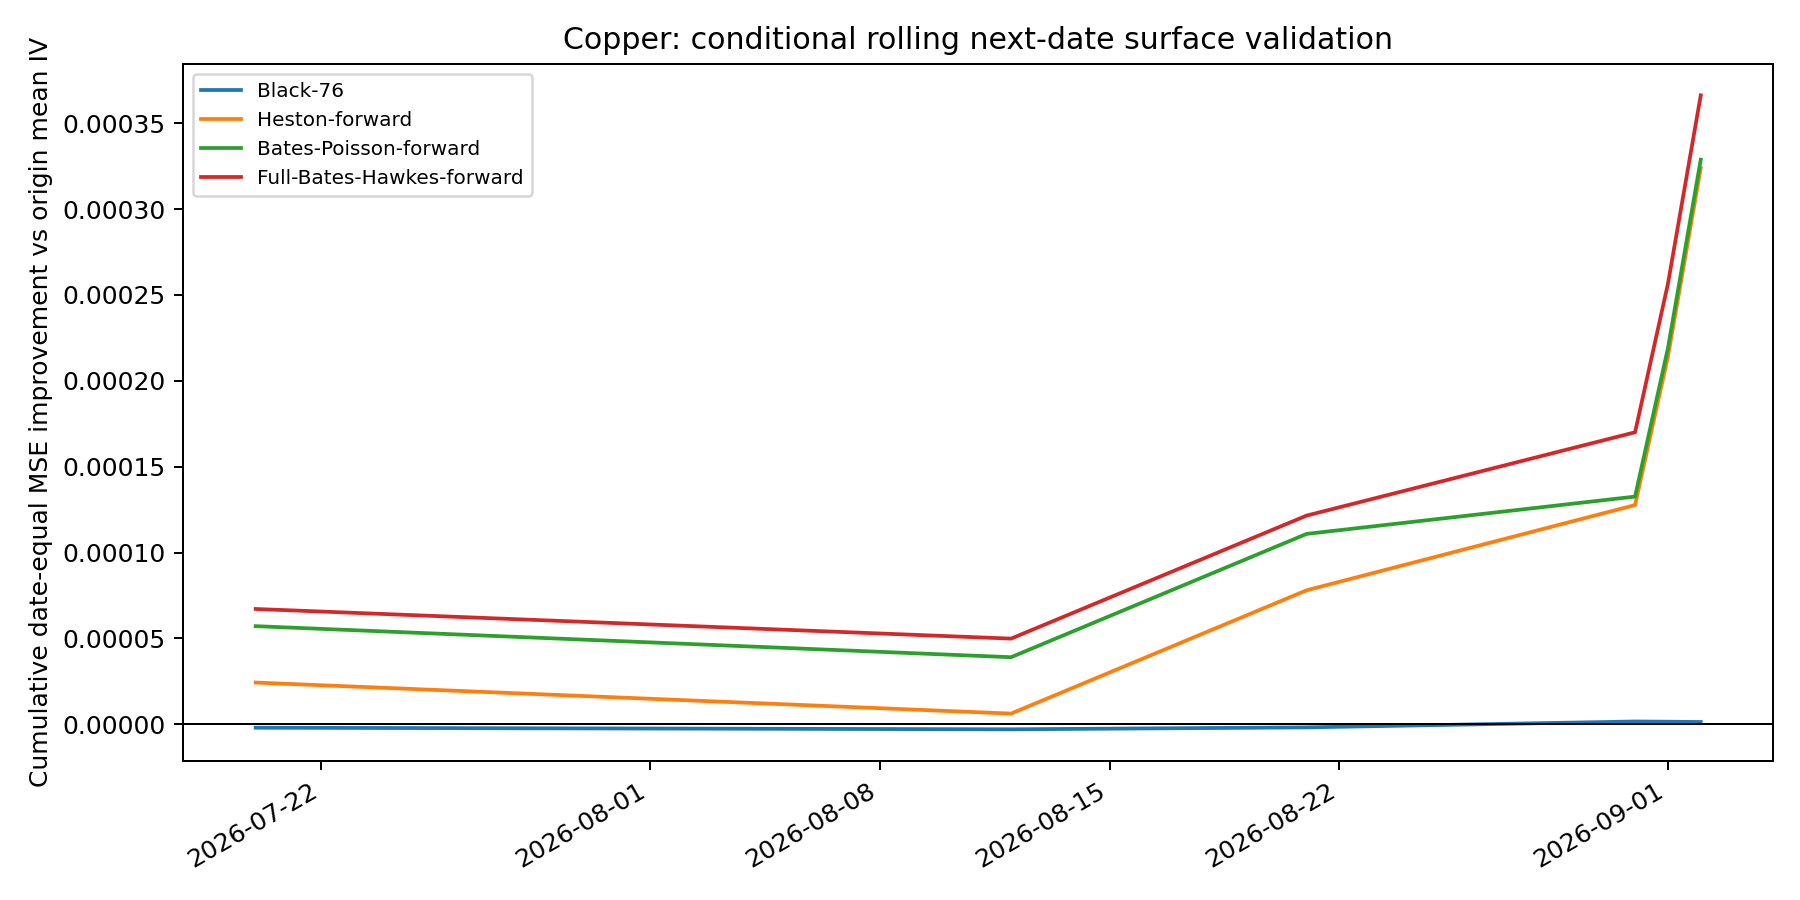
\includegraphics[width=.96\textwidth]{img/copper/copper_temporal_oos.png}
\caption{Cumulative date-equal MSE improvement against origin-mean IV. Only actual admitted targets enter; elapsed gaps are preserved. Positive improvement against this benchmark need not imply improvement against surface persistence.}
\label{fig:copper-temporal-oos}
\end{figure}
}{%
\gapbox{Historical copper acquisition and temporal validation are in progress.
The first static valuation is not temporally validated. Admit final coverage,
actual origin--target scores and the new paired valuation only from completed,
hash-verified local runs.}}
